\section{Partitionierung}

\section{Partitionierung}

\section{Partitionierung}

\section{Partitionierung}

\input{figures/partitionierung}

\subsection{Grundlagen}

\begin{itemize}
  \item ungerichtete Distanzadjazenzmatrix $\gls{Adist} \in \gls{R+}^{N \times N} = {\left(a\right)}_{ij}$
  \item (lokal) normalisierte ungerichtete Distanzadjazenzmatrix $\gls{Adistnorm} \in \gls{R+}^{N \times N} = {\left(\tilde a\right)}_{ij}$
  \item gerichtete Winkeladjazenzmatrix $\gls{Arad} \in \gls{R+}^{N \times N} = {\left(\alpha\right)}_{ij}$
  \item Input-Featurematrix $\gls{F} \in \gls{R}^{N \times X} = {\left(f\right)}_{ij}$
  \item Output-Featurematrix $\gls{Fout} \in \gls{R}^{N \times Y} = {\left(f^{\prime}\right)}_{ij}$
  \item Anzahl Partitionen $P \in \gls{N}$
  \item Gewichtstensor $\ma{W} \in \gls{R}^{\left(P + 1\right) \times X \times Y} = {\left(w\right)}_{ijw}$
\end{itemize}

\subsection{Faltung}

\begin{equation}
  f^{\prime}_{iy} = \sum_{x = 1}^X \tilde a_{ii} \cdot f_{ix} \cdot w_{\left(P +1\right)xy} \sum_{n = 1, n \neq i}^N \tilde a_{in} \cdot f_{nx} \cdot b^K_P\left(\alpha_{in}, x, y\right)
\end{equation}
wobei $b_P^K$ eine B-Spline-Kurve.

Es ist anzumerken, dass im Summanden der betrachtete Knoten übersprungen wird, da für diesen ein Wert in der Winkelmatrix keinen Sinn ergibt.
Er wird daher in der Faltung jeweils einzeln mit einem Gewicht multipliziert und dazuaddiert.

\subsection{B-Spline-Kurven}

$b_P^K \colon \left]0, 2\pi\right] \times \left\{1, \ldots, X \right\} \times \left\{1, \ldots, Y\right\} \to \gls{R}$ ist eine B-Spline-Kurve der Ordnung $K \in \gls{N}$ auf den Kantenwinkeln des Graphen.
Bemerke, dass wir $0$ für Winkel aussschließen und stattdessen den Winkel $2\pi$ benutzen, so dass wir nicht mit der Bedeutung von $0$ bei Adjazenzmatrizen in die Quere kommen.
\begin{equation}
  b_P^K\left(\alpha, x, y \right) = \sum_{p=1}^P w_{pxy} \cdot e_p^K\left(\alpha\right)
\end{equation}
wobei die Basisfunktion $e_p^K$ rekursiv über $K$ definiert ist mit Initialisierung
\begin{equation}
  e_p^1\left(\alpha\right) = \begin{cases}
    1, & \text{wenn }\alpha \in \left] t\left(p-1\right), t\left(p\right)\right]\text{,}\\
    0, & \text{sonst}
  \end{cases}
\end{equation}
und Rekursionsschritt
\begin{equation}
  e_p^k\left(\alpha\right) = \frac{\alpha - t\left(p - 1\right)}{t\left(p+k-2\right) - t\left(p - 1\right)} e_p^{k-1}\left(\alpha\right) + \frac{t\left(i\left(p + k - 1\right)\right) - \alpha}{t\left(p+k - 1\right) - t\left(p\right)} e_{i\left(p+1\right)}^{k-1}\left(\alpha\right)
\end{equation}
wobei $t \colon \gls{N} \to \gls{R}$ mit $t\left(p\right) = 2\pi\frac{p}{P}$ und $i\left(p\right) = \gls{modulo}\left(p-1, P\right) + 1$.
Es ist anzumerken, dass wir $t$ und $i$ dabei für den Rekursionsschritt über die Grenze $P$ hinaus definieren.
Das hilft uns, die B-Spline-Kurve \emph{kreisförmig} abzuschließen.

Je größer $K$ gesetzt wird, umso mehr Anteile anderer benachbarter Stützpunkte fließen in die Berechnung mit ein.
Die Größe von $K$ wird deshalb auch oft \emph{lokale Kontrollierbarkeit} genannt.

\subsubsection{Beispiel mit $P=4$}

\input{figures/bspline-basis}

\subsubsection{Effiziente Berechnung für $K=2$}

Wir können für $K=2$ die Basis-Berechnung durch
\begin{equation}
  e_p^2\left(\alpha\right) = \begin{cases}
    \min\left(\frac{P}{2\pi} \alpha - p + 1, 0\right), & \text{wenn }\alpha \leq t\left(p\right)\text{,}\\
    \min\left(-\frac{P}{2\pi} \alpha + p + 1, 0\right), & \text{sonst}
  \end{cases}
\end{equation}
vereinfachen.

\begin{proof}
  Aufsteigende Gerade der Dreiecksfunktion für $p$, $1 \leq p \leq P$, ist definiert durch
  \begin{equation}
    \frac{\alpha - t\left(p-1\right)}{t\left(p\right) - t\left(p-1\right)} = \frac{P\left(\alpha - t\left(p-1\right)\right)}{2\pi} = \frac{P\alpha - 2\pi\left(p-1\right)}{2\pi} = \frac{P}{2\pi}\alpha - p + 1.
  \end{equation}
  $\min \left(\frac{P}{2\pi} \alpha - p + 1, 0\right)$ beschreibt damit die linke Seite des Dreiecks.
  Analog für absteigende Gerade.
\end{proof}

Die Fallunterscheidung ist unnötig, wir können uns einfach immer für das Minimum der beiden entscheiden.
Die Grafik zeigt dies ziemlich eindeutig.
Das ergibt letztendlich
\begin{equation}
  e_p^2\left(\alpha\right) = \min \left( \min\left(\frac{P}{2\pi} \alpha - p + 1, 0\right), \min\left(-\frac{P}{2\pi} \alpha + p + 1, 0\right) \right)\text{.}
\end{equation}

\input{figures/bspline-basis-k-2}

Wir haben bisher noch nicht den \emph{Kreis} geschlossen mit unserer Formel.

Das können wir aber leicht tun, indem wir unsere absteigenden Geraden um $2\pi$ nach links verschieben und daraus wiederum das Minimum von $0$ ziehen.
Dann sind diese Geraden außer für $p = P$ im Gültigkeitsbereich der Funktion allesamt $0$.
Wir können demnach aus unserer bisherigen Formel und der verschobenen Gerade das Maximum ziehen.
Wir erhalten
\begin{equation}
\begin{split}
  e_p^2\left(\alpha\right) = \max \biggr( & \min \left( \min\left(\frac{P}{2\pi} \alpha - p + 1, 0\right), \min\left(-\frac{P}{2\pi} \alpha + p + 1, 0\right) \right),\\
  & \min \left(-\frac{P}{2\pi} \left( \alpha + 2\pi \right) + p + 1, 0\right) \biggr)\text{.}
\end{split}
\end{equation}

\subsection{Tensorimplementierung}

\begin{equation}
\begin{split}
  \gls{Fout} = & \ {\left(\gls{Adistnorm}\right)}_{ii} \cdot \gls{F} \cdot \ma{W}_{P+1}\\
  & + \sum_{p=1}^P \gls{Adistnorm} \gls{hadamard} e^K_p\left(\gls{Arad}\right) \cdot \gls{F} \cdot \ma{W}_{p}
\end{split}
\end{equation}

\gls{Adistnorm} enthält einmal nur die Diagonale und einmal alles ohne Diagonale.

\newpage


\subsection{Grundlagen}

\begin{itemize}
  \item ungerichtete Distanzadjazenzmatrix $\gls{Adist} \in \gls{R+}^{N \times N} = {\left(a\right)}_{ij}$
  \item (lokal) normalisierte ungerichtete Distanzadjazenzmatrix $\gls{Adistnorm} \in \gls{R+}^{N \times N} = {\left(\tilde a\right)}_{ij}$
  \item gerichtete Winkeladjazenzmatrix $\gls{Arad} \in \gls{R+}^{N \times N} = {\left(\alpha\right)}_{ij}$
  \item Input-Featurematrix $\gls{F} \in \gls{R}^{N \times X} = {\left(f\right)}_{ij}$
  \item Output-Featurematrix $\gls{Fout} \in \gls{R}^{N \times Y} = {\left(f^{\prime}\right)}_{ij}$
  \item Anzahl Partitionen $P \in \gls{N}$
  \item Gewichtstensor $\ma{W} \in \gls{R}^{\left(P + 1\right) \times X \times Y} = {\left(w\right)}_{ijw}$
\end{itemize}

\subsection{Faltung}

\begin{equation}
  f^{\prime}_{iy} = \sum_{x = 1}^X \tilde a_{ii} \cdot f_{ix} \cdot w_{\left(P +1\right)xy} \sum_{n = 1, n \neq i}^N \tilde a_{in} \cdot f_{nx} \cdot b^K_P\left(\alpha_{in}, x, y\right)
\end{equation}
wobei $b_P^K$ eine B-Spline-Kurve.

Es ist anzumerken, dass im Summanden der betrachtete Knoten übersprungen wird, da für diesen ein Wert in der Winkelmatrix keinen Sinn ergibt.
Er wird daher in der Faltung jeweils einzeln mit einem Gewicht multipliziert und dazuaddiert.

\subsection{B-Spline-Kurven}

$b_P^K \colon \left]0, 2\pi\right] \times \left\{1, \ldots, X \right\} \times \left\{1, \ldots, Y\right\} \to \gls{R}$ ist eine B-Spline-Kurve der Ordnung $K \in \gls{N}$ auf den Kantenwinkeln des Graphen.
Bemerke, dass wir $0$ für Winkel aussschließen und stattdessen den Winkel $2\pi$ benutzen, so dass wir nicht mit der Bedeutung von $0$ bei Adjazenzmatrizen in die Quere kommen.
\begin{equation}
  b_P^K\left(\alpha, x, y \right) = \sum_{p=1}^P w_{pxy} \cdot e_p^K\left(\alpha\right)
\end{equation}
wobei die Basisfunktion $e_p^K$ rekursiv über $K$ definiert ist mit Initialisierung
\begin{equation}
  e_p^1\left(\alpha\right) = \begin{cases}
    1, & \text{wenn }\alpha \in \left] t\left(p-1\right), t\left(p\right)\right]\text{,}\\
    0, & \text{sonst}
  \end{cases}
\end{equation}
und Rekursionsschritt
\begin{equation}
  e_p^k\left(\alpha\right) = \frac{\alpha - t\left(p - 1\right)}{t\left(p+k-2\right) - t\left(p - 1\right)} e_p^{k-1}\left(\alpha\right) + \frac{t\left(i\left(p + k - 1\right)\right) - \alpha}{t\left(p+k - 1\right) - t\left(p\right)} e_{i\left(p+1\right)}^{k-1}\left(\alpha\right)
\end{equation}
wobei $t \colon \gls{N} \to \gls{R}$ mit $t\left(p\right) = 2\pi\frac{p}{P}$ und $i\left(p\right) = \gls{modulo}\left(p-1, P\right) + 1$.
Es ist anzumerken, dass wir $t$ und $i$ dabei für den Rekursionsschritt über die Grenze $P$ hinaus definieren.
Das hilft uns, die B-Spline-Kurve \emph{kreisförmig} abzuschließen.

Je größer $K$ gesetzt wird, umso mehr Anteile anderer benachbarter Stützpunkte fließen in die Berechnung mit ein.
Die Größe von $K$ wird deshalb auch oft \emph{lokale Kontrollierbarkeit} genannt.

\subsubsection{Beispiel mit $P=4$}

\begin{center}
\begin{tikzpicture}
  \begin{axis}[xmax=4.5,
               xmin=0,
               ymin=0,
               ymax=1.25,
               xlabel={$\alpha$},
               ylabel={$e_p^1$},
               xtick={1, 2, 3, 4},
               xticklabels={$\frac{\pi}{2}$, $\pi$, $\frac{3\pi}{2}$, $2\pi$},
               ytick={1},
               axis equal,
               axis x line=center,
               axis y line=center,
               xlabel style={below right},
               ylabel style={above left},
               legend pos=outer north east]
    \addplot [ultra thick, brown] coordinates {(0,1)(1,1)};
    \addlegendentry{$p = 1$}
    \addplot [ultra thick, blue] coordinates {(1,1)(2,1)};
    \addlegendentry{$p = 2$}
    \addplot [ultra thick, red] coordinates {(2,1)(3,1)};
    \addlegendentry{$p = 3$}
    \addplot [ultra thick, green] coordinates {(3,1)(4,1)};
    \addlegendentry{$p = 4$}
  \end{axis}
\end{tikzpicture}
\end{center}

\begin{center}
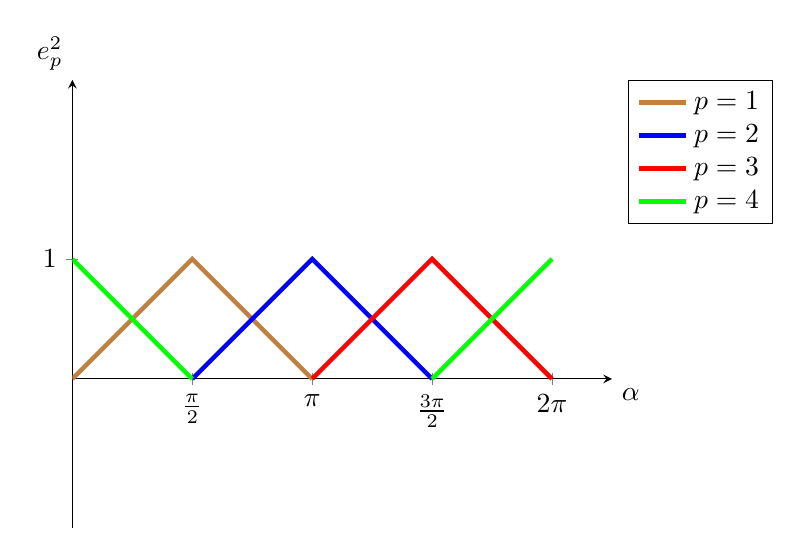
\begin{tikzpicture}
  \begin{axis}[xmax=4.5,
               xmin=0,
               ymin=0,
               ymax=1.25,
               xlabel={$\alpha$},
               ylabel={$e_p^2$},
               xtick={1, 2, 3, 4},
               xticklabels={$\frac{\pi}{2}$, $\pi$, $\frac{3\pi}{2}$, $2\pi$},
               ytick={1},
               axis equal,
               axis x line=center,
               axis y line=center,
               xlabel style={below right},
               ylabel style={above left},
               legend pos=outer north east]
    \addplot [ultra thick, brown] coordinates {(0,0)(1,1)(2,0)};
    \addlegendentry{$p = 1$}
    \addplot [ultra thick, blue] coordinates {(1,0)(2,1)(3,0)};
    \addlegendentry{$p = 2$}
    \addplot [ultra thick, red] coordinates {(2,0)(3,1)(4,0)};
    \addlegendentry{$p = 3$}
    \addplot [ultra thick, green] coordinates {(3,0)(4,1)};
    \addlegendentry{$p = 4$}
    \addplot [ultra thick, green] coordinates {(0,1)(1,0)};
  \end{axis}
\end{tikzpicture}
\end{center}


\subsubsection{Effiziente Berechnung für $K=2$}

Wir können für $K=2$ die Basis-Berechnung durch
\begin{equation}
  e_p^2\left(\alpha\right) = \begin{cases}
    \min\left(\frac{P}{2\pi} \alpha - p + 1, 0\right), & \text{wenn }\alpha \leq t\left(p\right)\text{,}\\
    \min\left(-\frac{P}{2\pi} \alpha + p + 1, 0\right), & \text{sonst}
  \end{cases}
\end{equation}
vereinfachen.

\begin{proof}
  Aufsteigende Gerade der Dreiecksfunktion für $p$, $1 \leq p \leq P$, ist definiert durch
  \begin{equation}
    \frac{\alpha - t\left(p-1\right)}{t\left(p\right) - t\left(p-1\right)} = \frac{P\left(\alpha - t\left(p-1\right)\right)}{2\pi} = \frac{P\alpha - 2\pi\left(p-1\right)}{2\pi} = \frac{P}{2\pi}\alpha - p + 1.
  \end{equation}
  $\min \left(\frac{P}{2\pi} \alpha - p + 1, 0\right)$ beschreibt damit die linke Seite des Dreiecks.
  Analog für absteigende Gerade.
\end{proof}

Die Fallunterscheidung ist unnötig, wir können uns einfach immer für das Minimum der beiden entscheiden.
Die Grafik zeigt dies ziemlich eindeutig.
Das ergibt letztendlich
\begin{equation}
  e_p^2\left(\alpha\right) = \min \left( \min\left(\frac{P}{2\pi} \alpha - p + 1, 0\right), \min\left(-\frac{P}{2\pi} \alpha + p + 1, 0\right) \right)\text{.}
\end{equation}

\begin{figure}
  \centering
  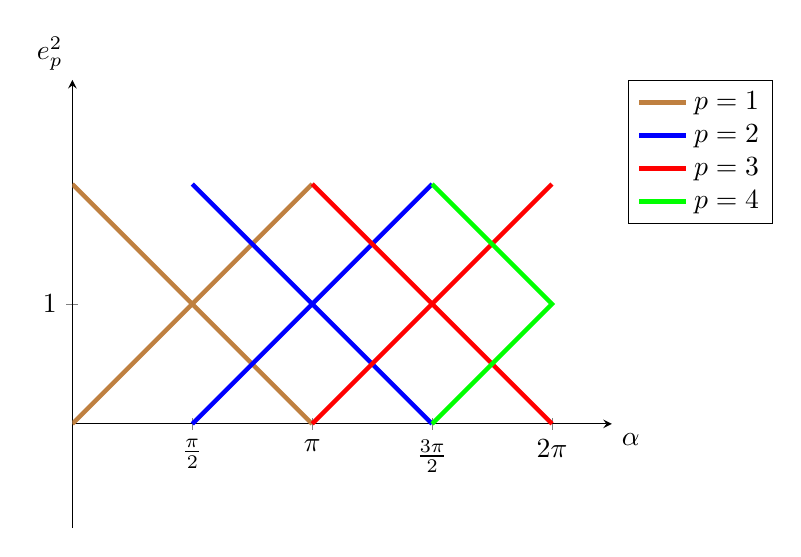
\begin{tikzpicture}
    \begin{axis}[xmax=4.5,
                 xmin=0,
                 ymin=0,
                 ymax=2,
                 xlabel={$\alpha$},
                 ylabel={$e_p^2$},
                 xtick={1, 2, 3, 4},
                 xticklabels={$\frac{\pi}{2}$, $\pi$, $\frac{3\pi}{2}$, $2\pi$},
                 ytick={1},
                 axis equal,
                 axis x line=center,
                 axis y line=center,
                 xlabel style={below right},
                 ylabel style={above left},
                 legend pos=outer north east]
      \addplot [ultra thick, brown] coordinates {(0,0)(2,2)(1,1)(0,2)(2,0)};
      \addlegendentry{$p = 1$}
      \addplot [ultra thick, blue] coordinates {(1,0)(3,2)(2,1)(1,2)(3,0)};
      \addlegendentry{$p = 2$}
      \addplot [ultra thick, red] coordinates {(2,0)(4,2)(3,1)(2,2)(4,0)};
      \addlegendentry{$p = 3$}
      \addplot [ultra thick, green] coordinates {(3,0)(4,1)(3,2)};
      \addlegendentry{$p = 4$}
    \end{axis}
  \end{tikzpicture}
\end{figure}


Wir haben bisher noch nicht den \emph{Kreis} geschlossen mit unserer Formel.

Das können wir aber leicht tun, indem wir unsere absteigenden Geraden um $2\pi$ nach links verschieben und daraus wiederum das Minimum von $0$ ziehen.
Dann sind diese Geraden außer für $p = P$ im Gültigkeitsbereich der Funktion allesamt $0$.
Wir können demnach aus unserer bisherigen Formel und der verschobenen Gerade das Maximum ziehen.
Wir erhalten
\begin{equation}
\begin{split}
  e_p^2\left(\alpha\right) = \max \biggr( & \min \left( \min\left(\frac{P}{2\pi} \alpha - p + 1, 0\right), \min\left(-\frac{P}{2\pi} \alpha + p + 1, 0\right) \right),\\
  & \min \left(-\frac{P}{2\pi} \left( \alpha + 2\pi \right) + p + 1, 0\right) \biggr)\text{.}
\end{split}
\end{equation}

\subsection{Tensorimplementierung}

\begin{equation}
\begin{split}
  \gls{Fout} = & \ {\left(\gls{Adistnorm}\right)}_{ii} \cdot \gls{F} \cdot \ma{W}_{P+1}\\
  & + \sum_{p=1}^P \gls{Adistnorm} \gls{hadamard} e^K_p\left(\gls{Arad}\right) \cdot \gls{F} \cdot \ma{W}_{p}
\end{split}
\end{equation}

\gls{Adistnorm} enthält einmal nur die Diagonale und einmal alles ohne Diagonale.

\newpage


\subsection{Grundlagen}

\begin{itemize}
  \item ungerichtete Distanzadjazenzmatrix $\gls{Adist} \in \gls{R+}^{N \times N} = {\left(a\right)}_{ij}$
  \item (lokal) normalisierte ungerichtete Distanzadjazenzmatrix $\gls{Adistnorm} \in \gls{R+}^{N \times N} = {\left(\tilde a\right)}_{ij}$
  \item gerichtete Winkeladjazenzmatrix $\gls{Arad} \in \gls{R+}^{N \times N} = {\left(\alpha\right)}_{ij}$
  \item Input-Featurematrix $\gls{F} \in \gls{R}^{N \times X} = {\left(f\right)}_{ij}$
  \item Output-Featurematrix $\gls{Fout} \in \gls{R}^{N \times Y} = {\left(f^{\prime}\right)}_{ij}$
  \item Anzahl Partitionen $P \in \gls{N}$
  \item Gewichtstensor $\ma{W} \in \gls{R}^{\left(P + 1\right) \times X \times Y} = {\left(w\right)}_{ijw}$
\end{itemize}

\subsection{Faltung}

\begin{equation}
  f^{\prime}_{iy} = \sum_{x = 1}^X \tilde a_{ii} \cdot f_{ix} \cdot w_{\left(P +1\right)xy} \sum_{n = 1, n \neq i}^N \tilde a_{in} \cdot f_{nx} \cdot b^K_P\left(\alpha_{in}, x, y\right)
\end{equation}
wobei $b_P^K$ eine B-Spline-Kurve.

Es ist anzumerken, dass im Summanden der betrachtete Knoten übersprungen wird, da für diesen ein Wert in der Winkelmatrix keinen Sinn ergibt.
Er wird daher in der Faltung jeweils einzeln mit einem Gewicht multipliziert und dazuaddiert.

\subsection{B-Spline-Kurven}

$b_P^K \colon \left]0, 2\pi\right] \times \left\{1, \ldots, X \right\} \times \left\{1, \ldots, Y\right\} \to \gls{R}$ ist eine B-Spline-Kurve der Ordnung $K \in \gls{N}$ auf den Kantenwinkeln des Graphen.
Bemerke, dass wir $0$ für Winkel aussschließen und stattdessen den Winkel $2\pi$ benutzen, so dass wir nicht mit der Bedeutung von $0$ bei Adjazenzmatrizen in die Quere kommen.
\begin{equation}
  b_P^K\left(\alpha, x, y \right) = \sum_{p=1}^P w_{pxy} \cdot e_p^K\left(\alpha\right)
\end{equation}
wobei die Basisfunktion $e_p^K$ rekursiv über $K$ definiert ist mit Initialisierung
\begin{equation}
  e_p^1\left(\alpha\right) = \begin{cases}
    1, & \text{wenn }\alpha \in \left] t\left(p-1\right), t\left(p\right)\right]\text{,}\\
    0, & \text{sonst}
  \end{cases}
\end{equation}
und Rekursionsschritt
\begin{equation}
  e_p^k\left(\alpha\right) = \frac{\alpha - t\left(p - 1\right)}{t\left(p+k-2\right) - t\left(p - 1\right)} e_p^{k-1}\left(\alpha\right) + \frac{t\left(i\left(p + k - 1\right)\right) - \alpha}{t\left(p+k - 1\right) - t\left(p\right)} e_{i\left(p+1\right)}^{k-1}\left(\alpha\right)
\end{equation}
wobei $t \colon \gls{N} \to \gls{R}$ mit $t\left(p\right) = 2\pi\frac{p}{P}$ und $i\left(p\right) = \gls{modulo}\left(p-1, P\right) + 1$.
Es ist anzumerken, dass wir $t$ und $i$ dabei für den Rekursionsschritt über die Grenze $P$ hinaus definieren.
Das hilft uns, die B-Spline-Kurve \emph{kreisförmig} abzuschließen.

Je größer $K$ gesetzt wird, umso mehr Anteile anderer benachbarter Stützpunkte fließen in die Berechnung mit ein.
Die Größe von $K$ wird deshalb auch oft \emph{lokale Kontrollierbarkeit} genannt.

\subsubsection{Beispiel mit $P=4$}

\begin{center}
\begin{tikzpicture}
  \begin{axis}[xmax=4.5,
               xmin=0,
               ymin=0,
               ymax=1.25,
               xlabel={$\alpha$},
               ylabel={$e_p^1$},
               xtick={1, 2, 3, 4},
               xticklabels={$\frac{\pi}{2}$, $\pi$, $\frac{3\pi}{2}$, $2\pi$},
               ytick={1},
               axis equal,
               axis x line=center,
               axis y line=center,
               xlabel style={below right},
               ylabel style={above left},
               legend pos=outer north east]
    \addplot [ultra thick, brown] coordinates {(0,1)(1,1)};
    \addlegendentry{$p = 1$}
    \addplot [ultra thick, blue] coordinates {(1,1)(2,1)};
    \addlegendentry{$p = 2$}
    \addplot [ultra thick, red] coordinates {(2,1)(3,1)};
    \addlegendentry{$p = 3$}
    \addplot [ultra thick, green] coordinates {(3,1)(4,1)};
    \addlegendentry{$p = 4$}
  \end{axis}
\end{tikzpicture}
\end{center}

\begin{center}
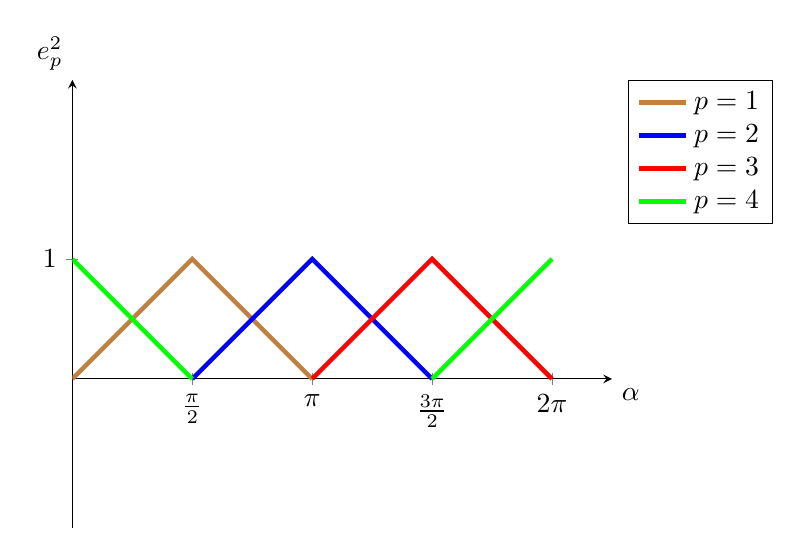
\begin{tikzpicture}
  \begin{axis}[xmax=4.5,
               xmin=0,
               ymin=0,
               ymax=1.25,
               xlabel={$\alpha$},
               ylabel={$e_p^2$},
               xtick={1, 2, 3, 4},
               xticklabels={$\frac{\pi}{2}$, $\pi$, $\frac{3\pi}{2}$, $2\pi$},
               ytick={1},
               axis equal,
               axis x line=center,
               axis y line=center,
               xlabel style={below right},
               ylabel style={above left},
               legend pos=outer north east]
    \addplot [ultra thick, brown] coordinates {(0,0)(1,1)(2,0)};
    \addlegendentry{$p = 1$}
    \addplot [ultra thick, blue] coordinates {(1,0)(2,1)(3,0)};
    \addlegendentry{$p = 2$}
    \addplot [ultra thick, red] coordinates {(2,0)(3,1)(4,0)};
    \addlegendentry{$p = 3$}
    \addplot [ultra thick, green] coordinates {(3,0)(4,1)};
    \addlegendentry{$p = 4$}
    \addplot [ultra thick, green] coordinates {(0,1)(1,0)};
  \end{axis}
\end{tikzpicture}
\end{center}


\subsubsection{Effiziente Berechnung für $K=2$}

Wir können für $K=2$ die Basis-Berechnung durch
\begin{equation}
  e_p^2\left(\alpha\right) = \begin{cases}
    \min\left(\frac{P}{2\pi} \alpha - p + 1, 0\right), & \text{wenn }\alpha \leq t\left(p\right)\text{,}\\
    \min\left(-\frac{P}{2\pi} \alpha + p + 1, 0\right), & \text{sonst}
  \end{cases}
\end{equation}
vereinfachen.

\begin{proof}
  Aufsteigende Gerade der Dreiecksfunktion für $p$, $1 \leq p \leq P$, ist definiert durch
  \begin{equation}
    \frac{\alpha - t\left(p-1\right)}{t\left(p\right) - t\left(p-1\right)} = \frac{P\left(\alpha - t\left(p-1\right)\right)}{2\pi} = \frac{P\alpha - 2\pi\left(p-1\right)}{2\pi} = \frac{P}{2\pi}\alpha - p + 1.
  \end{equation}
  $\min \left(\frac{P}{2\pi} \alpha - p + 1, 0\right)$ beschreibt damit die linke Seite des Dreiecks.
  Analog für absteigende Gerade.
\end{proof}

Die Fallunterscheidung ist unnötig, wir können uns einfach immer für das Minimum der beiden entscheiden.
Die Grafik zeigt dies ziemlich eindeutig.
Das ergibt letztendlich
\begin{equation}
  e_p^2\left(\alpha\right) = \min \left( \min\left(\frac{P}{2\pi} \alpha - p + 1, 0\right), \min\left(-\frac{P}{2\pi} \alpha + p + 1, 0\right) \right)\text{.}
\end{equation}

\begin{figure}
  \centering
  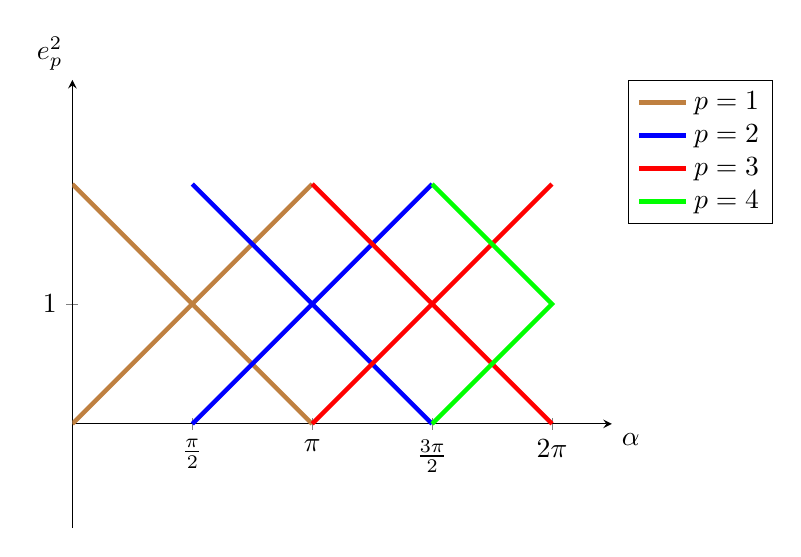
\begin{tikzpicture}
    \begin{axis}[xmax=4.5,
                 xmin=0,
                 ymin=0,
                 ymax=2,
                 xlabel={$\alpha$},
                 ylabel={$e_p^2$},
                 xtick={1, 2, 3, 4},
                 xticklabels={$\frac{\pi}{2}$, $\pi$, $\frac{3\pi}{2}$, $2\pi$},
                 ytick={1},
                 axis equal,
                 axis x line=center,
                 axis y line=center,
                 xlabel style={below right},
                 ylabel style={above left},
                 legend pos=outer north east]
      \addplot [ultra thick, brown] coordinates {(0,0)(2,2)(1,1)(0,2)(2,0)};
      \addlegendentry{$p = 1$}
      \addplot [ultra thick, blue] coordinates {(1,0)(3,2)(2,1)(1,2)(3,0)};
      \addlegendentry{$p = 2$}
      \addplot [ultra thick, red] coordinates {(2,0)(4,2)(3,1)(2,2)(4,0)};
      \addlegendentry{$p = 3$}
      \addplot [ultra thick, green] coordinates {(3,0)(4,1)(3,2)};
      \addlegendentry{$p = 4$}
    \end{axis}
  \end{tikzpicture}
\end{figure}


Wir haben bisher noch nicht den \emph{Kreis} geschlossen mit unserer Formel.

Das können wir aber leicht tun, indem wir unsere absteigenden Geraden um $2\pi$ nach links verschieben und daraus wiederum das Minimum von $0$ ziehen.
Dann sind diese Geraden außer für $p = P$ im Gültigkeitsbereich der Funktion allesamt $0$.
Wir können demnach aus unserer bisherigen Formel und der verschobenen Gerade das Maximum ziehen.
Wir erhalten
\begin{equation}
\begin{split}
  e_p^2\left(\alpha\right) = \max \biggr( & \min \left( \min\left(\frac{P}{2\pi} \alpha - p + 1, 0\right), \min\left(-\frac{P}{2\pi} \alpha + p + 1, 0\right) \right),\\
  & \min \left(-\frac{P}{2\pi} \left( \alpha + 2\pi \right) + p + 1, 0\right) \biggr)\text{.}
\end{split}
\end{equation}

\subsection{Tensorimplementierung}

\begin{equation}
\begin{split}
  \gls{Fout} = & \ {\left(\gls{Adistnorm}\right)}_{ii} \cdot \gls{F} \cdot \ma{W}_{P+1}\\
  & + \sum_{p=1}^P \gls{Adistnorm} \gls{hadamard} e^K_p\left(\gls{Arad}\right) \cdot \gls{F} \cdot \ma{W}_{p}
\end{split}
\end{equation}

\gls{Adistnorm} enthält einmal nur die Diagonale und einmal alles ohne Diagonale.

\newpage


\subsection{Grundlagen}

\begin{itemize}
  \item ungerichtete Distanzadjazenzmatrix $\gls{Adist} \in \gls{R+}^{N \times N} = {\left(a\right)}_{ij}$
  \item (lokal) normalisierte ungerichtete Distanzadjazenzmatrix $\gls{Adistnorm} \in \gls{R+}^{N \times N} = {\left(\tilde a\right)}_{ij}$
  \item gerichtete Winkeladjazenzmatrix $\gls{Arad} \in \gls{R+}^{N \times N} = {\left(\alpha\right)}_{ij}$
  \item Input-Featurematrix $\gls{F} \in \gls{R}^{N \times X} = {\left(f\right)}_{ij}$
  \item Output-Featurematrix $\gls{Fout} \in \gls{R}^{N \times Y} = {\left(f^{\prime}\right)}_{ij}$
  \item Anzahl Partitionen $P \in \gls{N}$
  \item Gewichtstensor $\ma{W} \in \gls{R}^{\left(P + 1\right) \times X \times Y} = {\left(w\right)}_{ijw}$
\end{itemize}

\subsection{Faltung}

\begin{equation}
  f^{\prime}_{iy} = \sum_{x = 1}^X \tilde a_{ii} \cdot f_{ix} \cdot w_{\left(P +1\right)xy} \sum_{n = 1, n \neq i}^N \tilde a_{in} \cdot f_{nx} \cdot b^K_P\left(\alpha_{in}, x, y\right)
\end{equation}
wobei $b_P^K$ eine B-Spline-Kurve.
\todo{$a_{ii}$ kann raus, da immer $1$}

Es ist anzumerken, dass im Summanden der betrachtete Knoten übersprungen wird, da für diesen ein Wert in der Winkelmatrix keinen Sinn ergibt.
Er wird daher in der Faltung jeweils einzeln mit einem Gewicht multipliziert und dazuaddiert.

\subsection{B-Spline-Kurven}

$b_P^K \colon \left]0, 2\pi\right] \times \left\{1, \ldots, X \right\} \times \left\{1, \ldots, Y\right\} \to \gls{R}$ ist eine B-Spline-Kurve der Ordnung $K \in \gls{N}$ auf den Kantenwinkeln des Graphen.
Bemerke, dass wir $0$ für Winkel aussschließen und stattdessen den Winkel $2\pi$ benutzen, so dass wir nicht mit der Bedeutung von $0$ bei Adjazenzmatrizen in die Quere kommen.
\begin{equation}
  b_P^K\left(\alpha, x, y \right) = \sum_{p=1}^P w_{pxy} \cdot e_p^K\left(\alpha\right)
\end{equation}
wobei die Basisfunktion $e_p^K$ rekursiv über $K$ definiert ist mit Initialisierung
\begin{equation}
  e_p^1\left(\alpha\right) = \begin{cases}
    1, & \text{wenn }\alpha \in \left] t\left(p-1\right), t\left(p\right)\right]\text{,}\\
    0, & \text{sonst}
  \end{cases}
\end{equation}
und Rekursionsschritt
\begin{equation}
  e_p^k\left(\alpha\right) = \frac{\alpha - t\left(p - 1\right)}{t\left(p+k-2\right) - t\left(p - 1\right)} e_p^{k-1}\left(\alpha\right) + \frac{t\left(i\left(p + k - 1\right)\right) - \alpha}{t\left(p+k - 1\right) - t\left(p\right)} e_{i\left(p+1\right)}^{k-1}\left(\alpha\right)
\end{equation}
wobei $t \colon \gls{N} \to \gls{R}$ mit $t\left(p\right) = 2\pi\frac{p}{P}$ und $i\left(p\right) = \gls{modulo}\left(p-1, P\right) + 1$.
Es ist anzumerken, dass wir $t$ und $i$ dabei für den Rekursionsschritt über die Grenze $P$ hinaus definieren.
Das hilft uns, die B-Spline-Kurve \emph{kreisförmig} abzuschließen.

Je größer $K$ gesetzt wird, umso mehr Anteile anderer benachbarter Stützpunkte fließen in die Berechnung mit ein.
Die Größe von $K$ wird deshalb auch oft \emph{lokale Kontrollierbarkeit} genannt.

\subsubsection{Beispiel mit $P=4$}

\begin{center}
\begin{tikzpicture}
  \begin{axis}[xmax=4.5,
               xmin=0,
               ymin=0,
               ymax=1.25,
               xlabel={$\alpha$},
               ylabel={$e_p^1$},
               xtick={1, 2, 3, 4},
               xticklabels={$\frac{\pi}{2}$, $\pi$, $\frac{3\pi}{2}$, $2\pi$},
               ytick={1},
               axis equal,
               axis x line=center,
               axis y line=center,
               xlabel style={below right},
               ylabel style={above left},
               legend pos=outer north east]
    \addplot [ultra thick, brown] coordinates {(0,1)(1,1)};
    \addlegendentry{$p = 1$}
    \addplot [ultra thick, blue] coordinates {(1,1)(2,1)};
    \addlegendentry{$p = 2$}
    \addplot [ultra thick, red] coordinates {(2,1)(3,1)};
    \addlegendentry{$p = 3$}
    \addplot [ultra thick, green] coordinates {(3,1)(4,1)};
    \addlegendentry{$p = 4$}
  \end{axis}
\end{tikzpicture}
\end{center}

\begin{center}
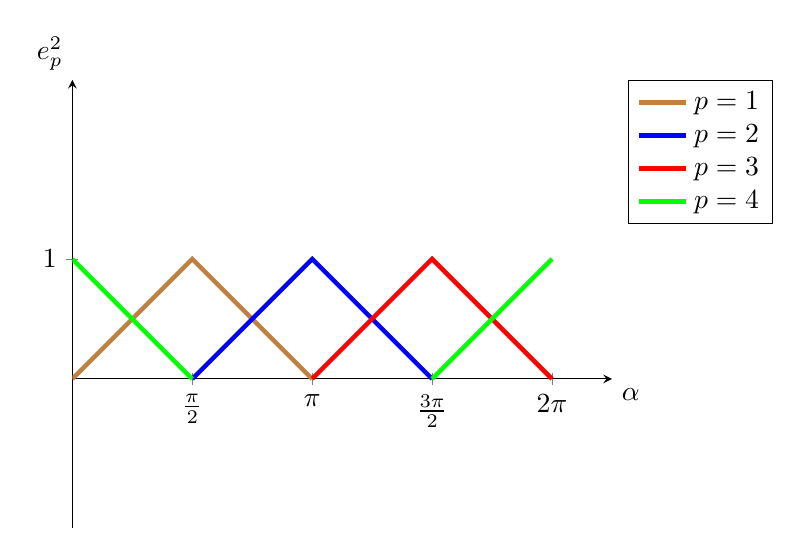
\begin{tikzpicture}
  \begin{axis}[xmax=4.5,
               xmin=0,
               ymin=0,
               ymax=1.25,
               xlabel={$\alpha$},
               ylabel={$e_p^2$},
               xtick={1, 2, 3, 4},
               xticklabels={$\frac{\pi}{2}$, $\pi$, $\frac{3\pi}{2}$, $2\pi$},
               ytick={1},
               axis equal,
               axis x line=center,
               axis y line=center,
               xlabel style={below right},
               ylabel style={above left},
               legend pos=outer north east]
    \addplot [ultra thick, brown] coordinates {(0,0)(1,1)(2,0)};
    \addlegendentry{$p = 1$}
    \addplot [ultra thick, blue] coordinates {(1,0)(2,1)(3,0)};
    \addlegendentry{$p = 2$}
    \addplot [ultra thick, red] coordinates {(2,0)(3,1)(4,0)};
    \addlegendentry{$p = 3$}
    \addplot [ultra thick, green] coordinates {(3,0)(4,1)};
    \addlegendentry{$p = 4$}
    \addplot [ultra thick, green] coordinates {(0,1)(1,0)};
  \end{axis}
\end{tikzpicture}
\end{center}


\subsubsection{Effiziente Berechnung für $K=1$}

Eigentlich ist nicht viel zu tun.
Wir suchen lediglich eine effiziente Implementierung für $e_p^1\left(\alpha\right)$, die auch von TensorFlow verstanden wird und ableitbar ist.
Es zeigt sich, dass $e_p^1\left(\alpha\right) = 1$ genau dann, wenn $\alpha > 2\pi\frac{p-1}{P}$ und $\alpha \leq 2\pi\frac{p}{P}$.
Vereinfact damit
\begin{equation}
  0 < \frac{P}{2\pi}\alpha + p + 1 \leq 1.
\end{equation}
Es bleibt die Ungleichungsüberprüfung.

\subsubsection{Effiziente Berechnung für $K=2$}

Wir können für $K=2$ die Basis-Berechnung durch
\begin{equation}
  e_p^2\left(\alpha\right) = \begin{cases}
    \max\left(\frac{P}{2\pi} \alpha - p + 1, 0\right), & \text{wenn }\alpha \leq t\left(p\right)\text{,}\\
    \max\left(-\frac{P}{2\pi} \alpha + p + 1, 0\right), & \text{sonst}
  \end{cases}
\end{equation}
vereinfachen.

\begin{proof}
  Aufsteigende Gerade der Dreiecksfunktion für $p$, $1 \leq p \leq P$, ist definiert durch
  \begin{equation}
    \frac{\alpha - t\left(p-1\right)}{t\left(p\right) - t\left(p-1\right)} = \frac{P\left(\alpha - t\left(p-1\right)\right)}{2\pi} = \frac{P\alpha - 2\pi\left(p-1\right)}{2\pi} = \frac{P}{2\pi}\alpha - p + 1.
  \end{equation}
  $\max \left(\frac{P}{2\pi} \alpha - p + 1, 0\right)$ beschreibt damit die linke Seite der Dreiecksfunktion.
  Analog für absteigende Gerade.
\end{proof}

Die Fallunterscheidung ist unnötig, wir können uns einfach immer für das Minimum der beiden entscheiden.
Die Grafik zeigt dies ziemlich eindeutig.
Das ergibt letztendlich
\begin{equation}
  e_p^2\left(\alpha\right) = \min \left( \max\left(\frac{P}{2\pi} \alpha - p + 1, 0\right), \max\left(-\frac{P}{2\pi} \alpha + p + 1, 0\right) \right)\text{.}
\end{equation}

\begin{figure}
  \centering
  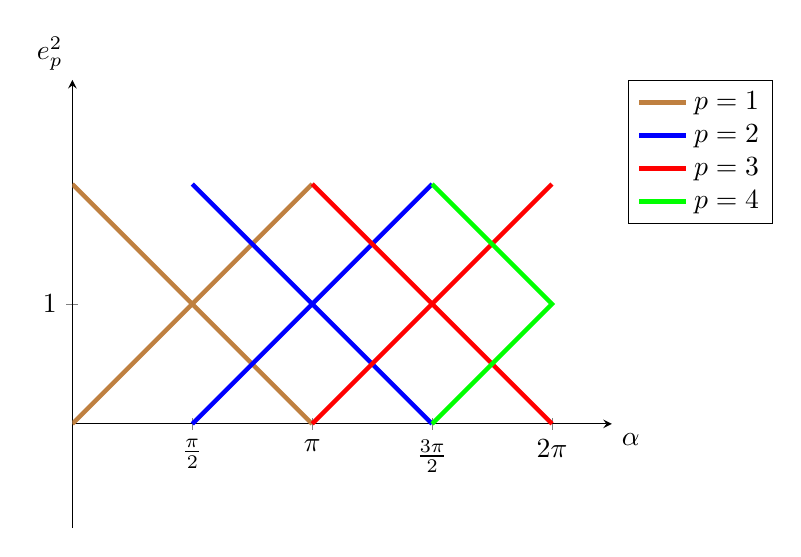
\begin{tikzpicture}
    \begin{axis}[xmax=4.5,
                 xmin=0,
                 ymin=0,
                 ymax=2,
                 xlabel={$\alpha$},
                 ylabel={$e_p^2$},
                 xtick={1, 2, 3, 4},
                 xticklabels={$\frac{\pi}{2}$, $\pi$, $\frac{3\pi}{2}$, $2\pi$},
                 ytick={1},
                 axis equal,
                 axis x line=center,
                 axis y line=center,
                 xlabel style={below right},
                 ylabel style={above left},
                 legend pos=outer north east]
      \addplot [ultra thick, brown] coordinates {(0,0)(2,2)(1,1)(0,2)(2,0)};
      \addlegendentry{$p = 1$}
      \addplot [ultra thick, blue] coordinates {(1,0)(3,2)(2,1)(1,2)(3,0)};
      \addlegendentry{$p = 2$}
      \addplot [ultra thick, red] coordinates {(2,0)(4,2)(3,1)(2,2)(4,0)};
      \addlegendentry{$p = 3$}
      \addplot [ultra thick, green] coordinates {(3,0)(4,1)(3,2)};
      \addlegendentry{$p = 4$}
    \end{axis}
  \end{tikzpicture}
\end{figure}


Wir haben bisher noch nicht den \emph{Kreis} geschlossen mit unserer Formel.

Das können wir aber leicht tun, indem wir unsere absteigenden Geraden um $2\pi$ nach links verschieben und daraus wiederum das Maximum von $0$ ziehen.
Dann sind diese Geraden außer für $p = P$ im Gültigkeitsbereich der Funktion allesamt $0$.
Wir können demnach aus unserer bisherigen Formel und der verschobenen Gerade das Maximum ziehen.
Wir erhalten
\begin{equation}
\begin{split}
  e_p^2\left(\alpha\right) = \max \biggr( & \min \left( \max\left(\frac{P}{2\pi} \alpha - p + 1, 0\right), \max\left(-\frac{P}{2\pi} \alpha + p + 1, 0\right) \right),\\
  & \max \left(-\frac{P}{2\pi} \left( \alpha + 2\pi \right) + p + 1, 0\right) \biggr)\text{.}
\end{split}
\end{equation}

\subsection{Tensorimplementierung}

\begin{equation}
\begin{split}
  \gls{Fout} = & \ {\left(\gls{Adistnorm}\right)}_{ii} \cdot \gls{F} \cdot \ma{W}_{P+1}\\
  & + \sum_{p=1}^P \gls{Adistnorm} \gls{hadamard} e^K_p\left(\gls{Arad}\right) \cdot \gls{F} \cdot \ma{W}_{p}
\end{split}
\end{equation}
mit $e_p^K(0) = 0$.
Elementweise Multiplikation mit dünnbesetzten Matrizen \texttt{sparse\_multiply} ist in TensorFlow nicht implementiert.
Es kann aber intern auf den Daten von dünnbesetzten Matrizen eine elementweise Multiplikation angewendet werden.
So kann die Faltung ohne Preprocessing implementiert werden.

\todo{$p$ soll bei $0$ anfangen}
\todo{$A_{ii}$ kann raus, da immer $1$}

\newpage
